\documentclass[10pt]{article}

\usepackage{amssymb,amsmath}
\usepackage[T1]{fontenc}
\usepackage{cite}
\usepackage[table,xcdraw]{xcolor}
\usepackage[utf8]{inputenc}
\usepackage{esdiff}
\usepackage{braket}
\usepackage[version=3]{mhchem}
\usepackage{verbatim}

\usepackage{siunitx}
\usepackage{graphicx,subcaption,subfig,float, multicol, tabularx}
%\usepackage{fullpage}

\renewcommand{\v}[1]{\mathbf{#1}}


\title{Modeling of biological systems, exercises}
\author{Markus Rauhalahti\\
	markus.rauhalahti@helsinki.fi}

\begin{document}
\maketitle
\tableofcontents

\begin{abstract}
	\noindent Exercises for the Modeling of Biological Systems course, University of Helsinki
	\begin{enumerate}
	\item Fitting of a Ryckaert-Bellemans potential to HF/DFT results
	\item Calculation of RESP charges
	\end{enumerate}
\end{abstract}

\newpage



\section{Dihedral parameters}

\subsection{Constrained scan}

The O-C-C-O dihedral angle was scanned from 0 to 180 degrees at 10 degree intervals, requiring 18 geometry optimizations per level of theory. Altogether 32 geometry optimizations would be needed, which would be slow using the aug-cc-pVTZ basis set.

For this reason, the geometries were optimized using the  PBEh-3c method, which is a fast and accurate method for molecular geometries\cite{pbeh3c}. It combines the PBEh density functional with three empirical corrections (3c) and a minimal basis set. These dihedral scans were performed using the ORCA 4.0.1 program\cite{orca}.

The input and output files for the scan are in \texttt{.qc\_calculations/scan/pbeh-3c}

\subsection{Single point calculations}


The single point energies of the obtained structures were computed with the HF and B3LYP\cite{b3lyp1, b3lyp2} SCF-methods with the aug-cc-pVTZ\cite{augccpvtz} basis set. The PBEh-3c orbitals were read to speed up the SCF convergance. The input and output files for these calculations are in \texttt{.qc\_calculations/scan/\{b3lyp,hf\}}. Single point calculations were also done using the MMFF94\cite{mmff94} force field using the Open Babel library\cite{openbabel}.

The barrier height $\mathcal{E}$ is defined as the energy relative to the energy of the most stable structure:

\begin{align}
\mathcal{E} &= E - \min (E)
\end{align}

The barrier heights for the PBEh-3c, HF, B3LYP quantum chemical methods and the MMFF94 force field are shown in figure \ref{fig:scan}.

\begin{figure}[ht!]
\centering
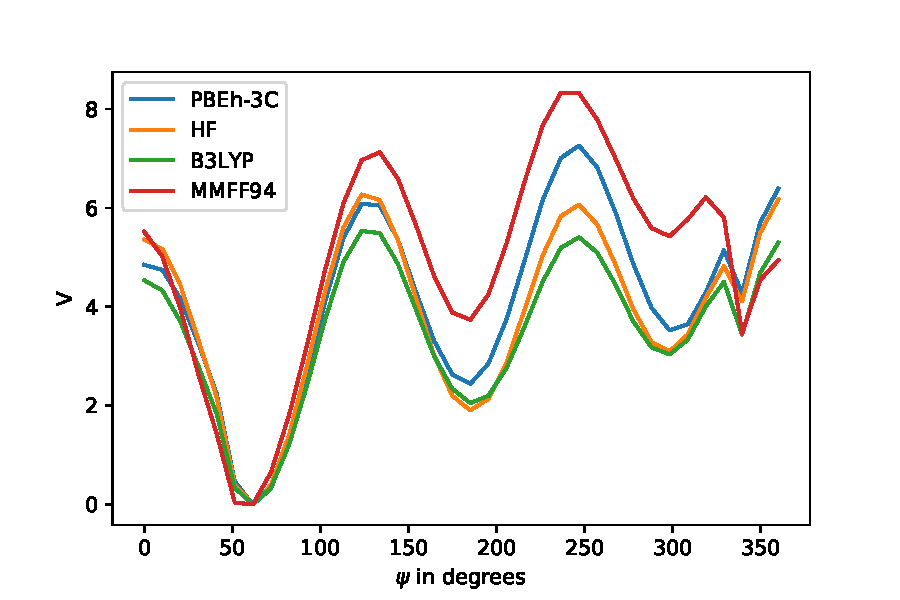
\includegraphics[width=0.7\linewidth]{fig/scan}
\caption{Energy (in kcal/mol) relative to the lowest energy geometry as a function of the dihedral angle (in degrees) with the PBEh-3c, HF, B3LYP quantum chemical methods and with the MMFF94 force field.}
\label{fig:scan}
\end{figure}

One can see that the the barriers are qualitatively very similar. The MMFF94 predicts too large barrier hights relative to the minimum energy. The difference between B3LYP and PBEh-3C may be accounted by the lack of dispersion correction of the B3LYP/aug-cc-pVTZ method.

\subsection{Fitting the potential}

The torsional energy was substracted from the total energy of the MMFF94 force field calculations:

\begin{align}
E_{\text{MD-tors}} &= E_{\text{MD}} - E_{\text{tors}}\\
\end{align}

The barrier heights of this were then substracted from the barrier heights obtained using the B3LYP and SCF methods, yielding $V_{\text{fit}}$. 

The Ryckaert-Bellemans potential is a 5th order trigonometric polynomial. 

\begin{align}
V_{rb}(\phi_{ijkl}) = \sum_{n=0}^5 C_n (\cos (\p si))^n
\end{align}

It was fit using the calculated $(V_{\text{fit}}, \phi)$ pairs using the $polyfit$ function of the $numpy$ library \cite{numpy}. The fitting, data manipulation, and visualizations are all contained in the \texttt{./analysis/potential\_fit.ipynb} Jupyter notebook\footnote{Also as a pdf, \texttt{\texttt{./analysis/potential\_fit.pdf}} }. The expansion coefficients $C_n$ are tabulated in table 1 and the Ryckaert-Bellemans  potentials as the function of dihedral angle are shown in figure \ref{fig:v_rb}.

\begin{table}[ht!]
	\centering
	\label{my-label}
	\begin{tabular}{ccc}
		Coefficient & B3LYP  &      HF       \\
		$C_1$ & 1.563306 &  1.486257 \\
		$C_2$ & 1.668620 &  1.575792 \\
		$C_3$ &-8.396610 & -9.882902 \\
		$C_4$ & 1.109764 &  1.209000 \\
		$C_5$ & 3.310302 &  4.355467 \\
		$C_6$ & 1.543540 &  1.830176
	\end{tabular}
	\caption{Fitted coefficients $C_n$ of the RB potential.}
\end{table}

\begin{figure}[th!]
\centering
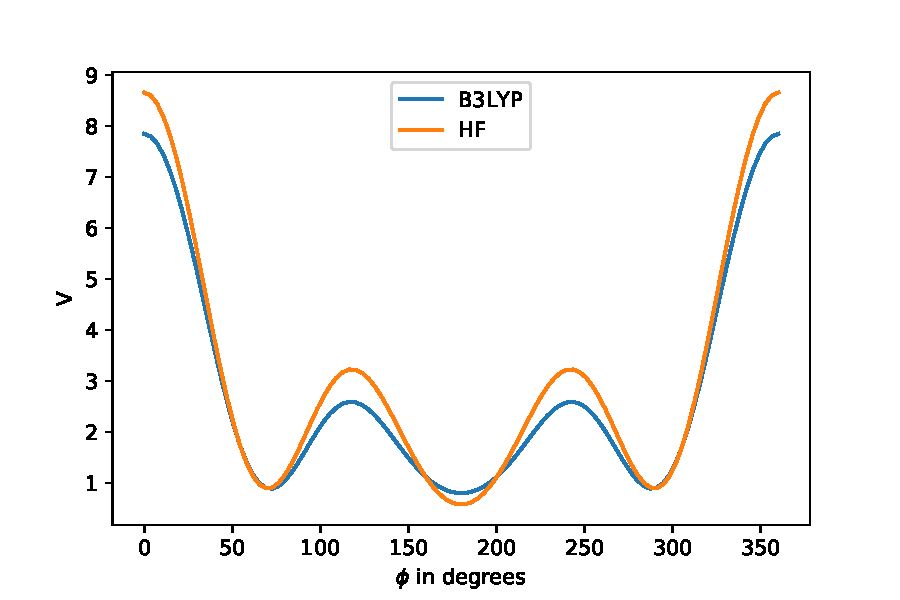
\includegraphics[width=0.7\linewidth]{fig/v_rb}
\caption{Ryckaert-Bellemans potential (in kcal/mol) as a function of dihedral angle.}
\label{fig:v_rb}
\end{figure}



\newpage


\section{RESP charges}

The RESP charges were calculated with Turbomole 7.2 using the B3LYP and SCF methods using the PBEh-3c geometries of the minimum energy structure. The input and output files are in \texttt{./qc\_calculations/resp/{b3lyp,hf}}. They are tabulated in table \ref{fig:resp} and shown in figure \ref{fig:resp}.

\begin{table}[ht!]
	\centering
	\label{resp}
	\begin{tabular}{llll} \hline
		atom & B3LYP & HF        &           \\ \hline
		1C &    0.204987  & 0.222241  \\
		2C &    0.37251   & 0.403284  \\
		3C &    -0.385143 & -0.406909 \\
		4H &    0.103488  & 0.107139  \\
		5H &    0.086909  & 0.091056  \\
		6H &    0.101354  & 0.110429  \\
		7O &    -0.662389 & -0.704385 \\
		8H &    -0.043494 & -0.044339 \\
		9H &    0.398354  & 0.417985  \\
		10O &   -0.597586 & -0.637468 \\
		11H &   0.000034  & 0.001739  \\
		12H &   0.034103  & 0.031094  \\
		13H &   0.386872  & 0.408134 \\ \hline
	\end{tabular}
	\caption{RESP charges using the B3LYP and HF methods with aug-cc-pVTZ basis set.}
\end{table}

\begin{figure}[ht!]
\centering
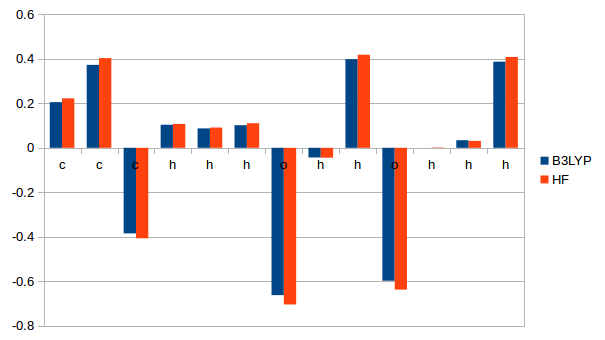
\includegraphics[width=0.8\linewidth]{fig/resp}
\caption{RESP charges using the B3LYP and HF methods with aug-cc-pVTZ basis set.}
\label{fig:resp}
\end{figure}


\bibliographystyle{unsrt}
\bibliography{ref}

\end{document}